\section{Scale-up Server Scalalbility}


\begin{figure*}[tb]
    \centering
    \begin{subfigure}[b]{0.20\textwidth}
        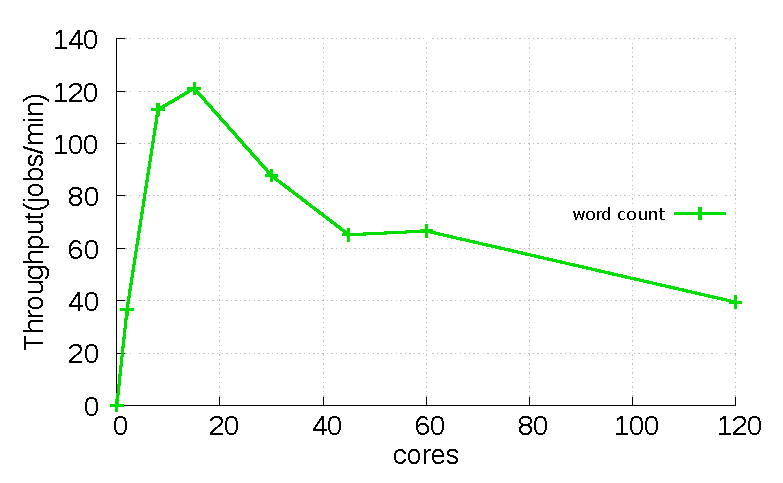
\includegraphics[width=1.4in]{graph/wc.eps}
        \caption{Word Count}
    \end{subfigure}%
    \begin{subfigure}[b]{0.20\textwidth}
        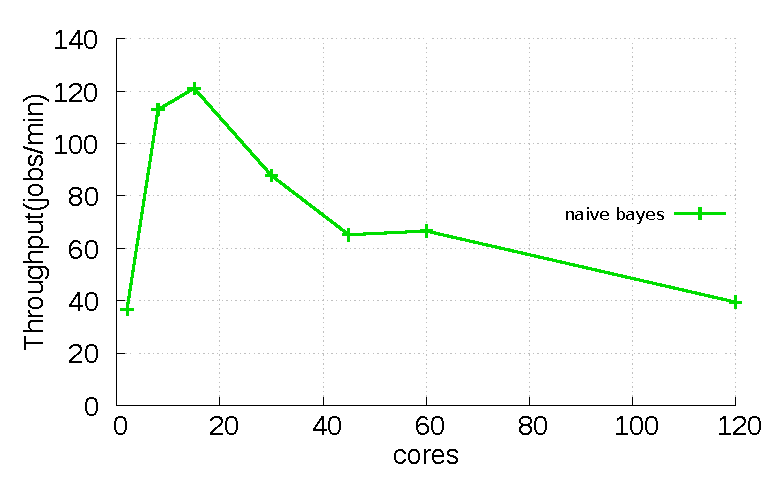
\includegraphics[width=1.4in]{graph/nb.eps}
        \caption{Naive Basian}
    \end{subfigure}%
    \begin{subfigure}[b]{0.20\textwidth}
        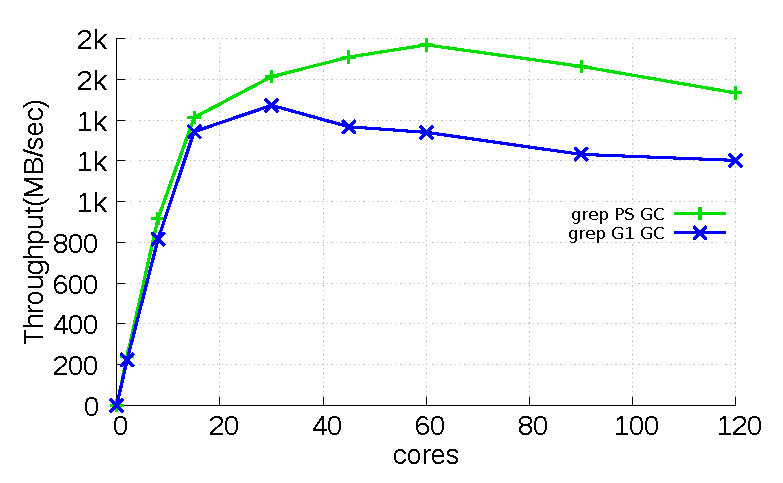
\includegraphics[width=1.4in]{graph/grep.eps}
        \caption{Grep}
    \end{subfigure}%
        \begin{subfigure}[b]{0.20\textwidth}
        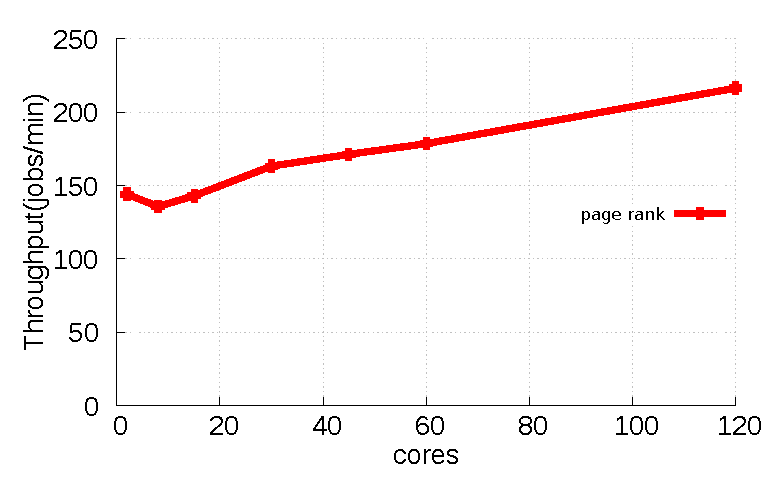
\includegraphics[width=1.4in]{graph/pagerank.eps}
        \caption{Pagerank}
    \end{subfigure}%
        \begin{subfigure}[b]{0.20\textwidth}
        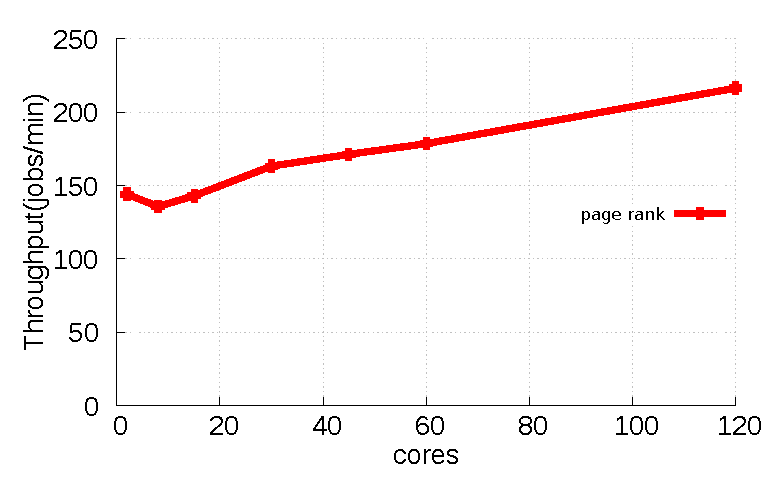
\includegraphics[width=1.4in]{graph/pagerank.eps}
        \caption{Pagerank}
    \end{subfigure}
    \caption{CPU utilization on 120 core.}
    \label{fig:utilization}
\end{figure*}



\begin{figure*}[tb]
    \centering
    \begin{subfigure}[b]{0.20\textwidth}
        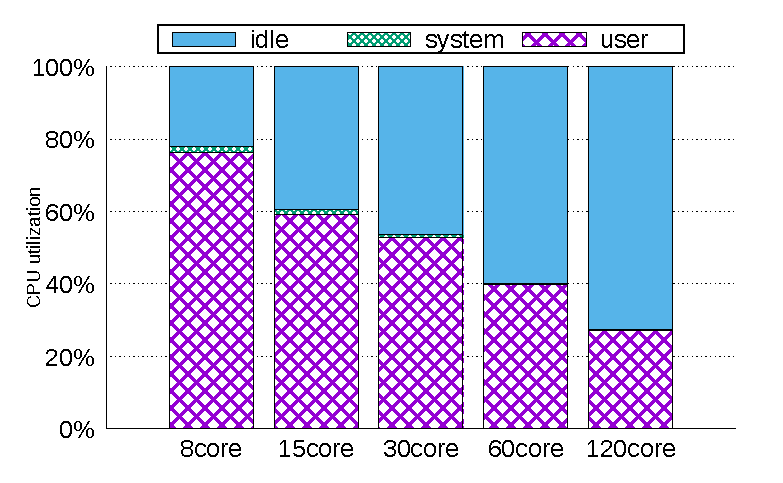
\includegraphics[width=1.4in]{graph/wc_cpuutils.eps}
        \caption{Word Count}
    \end{subfigure}%
    \begin{subfigure}[b]{0.20\textwidth}
        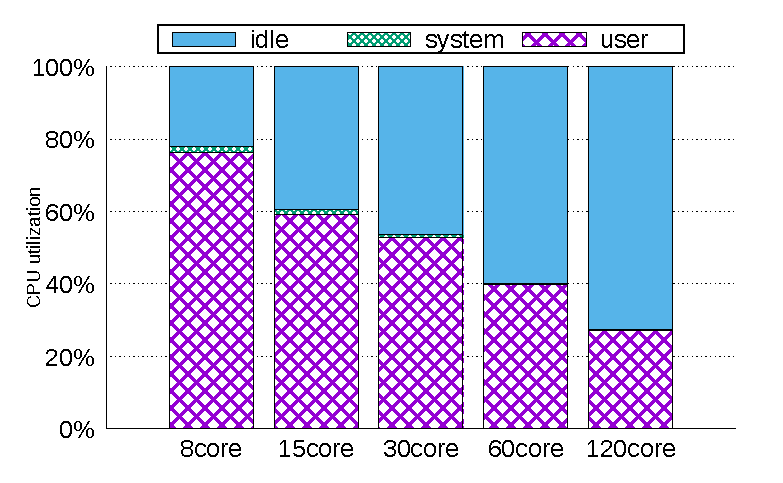
\includegraphics[width=1.4in]{graph/wc_cpuutils.eps}
        \caption{Naive Basian}
    \end{subfigure}%
    \begin{subfigure}[b]{0.20\textwidth}
        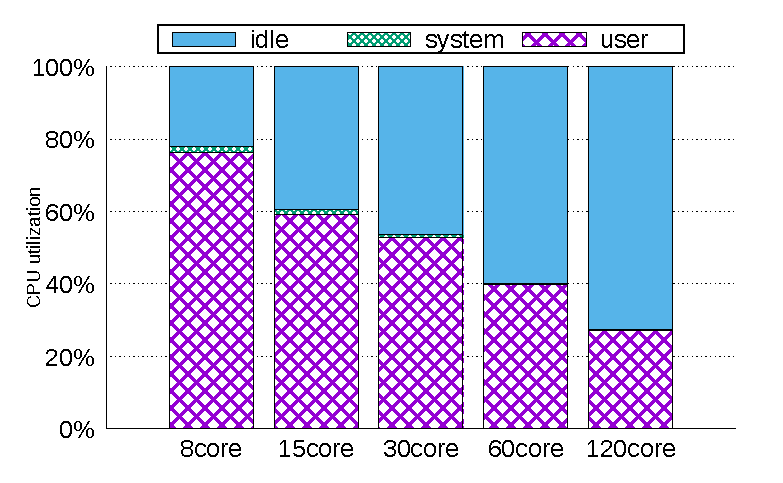
\includegraphics[width=1.4in]{graph/wc_cpuutils.eps}
        \caption{Grep}
    \end{subfigure}%
        \begin{subfigure}[b]{0.20\textwidth}
        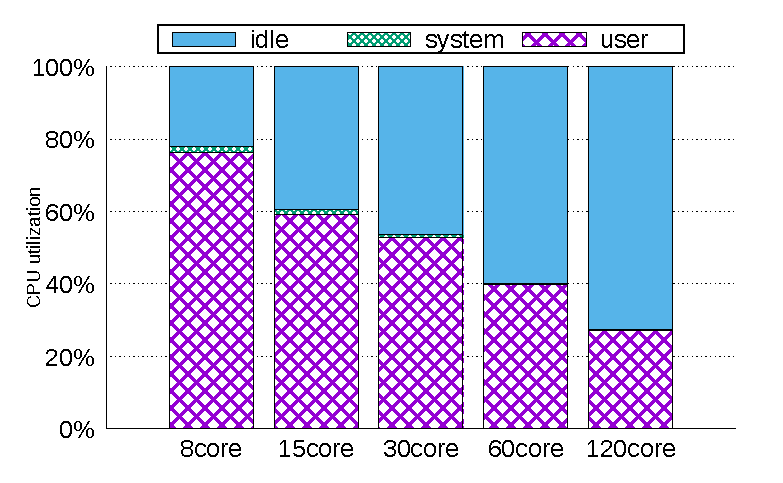
\includegraphics[width=1.4in]{graph/wc_cpuutils.eps}
        \caption{Pagerank}
    \end{subfigure}%
        \begin{subfigure}[b]{0.20\textwidth}
        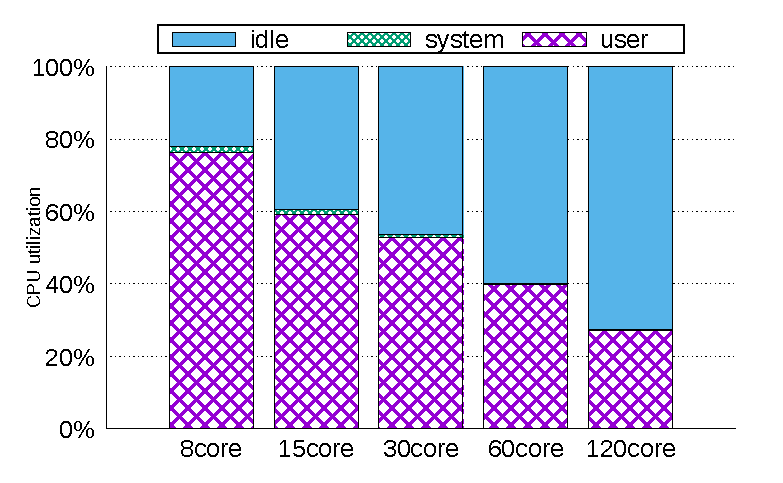
\includegraphics[width=1.4in]{graph/wc_cpuutils.eps}
        \caption{Pagerank}
    \end{subfigure}
        \centering
    \caption{CPU utilization on 120 core.}
    \label{fig:utilization}
\end{figure*}
Figure~\ref{fig:utilization}(a)) since it waits to acquire



%$$$$$$$$$$$$$$$$$$$$$$$$$$$$$$$$$$$$$$$$$$$$$$$$$$$$$$$$$$$$$$$$$$$$$$$$$$$$$$$$
%$$$$$$$$$$$$$$$$$$$$$$$$$$$$$$$$$$$$$$$$$$$$$$$$$$$$$$$$$$$$$$$$$$$$$$$$$$$$$$$$
% 이번 장에 대한 설명
%$$$$$$$$$$$$$$$$$$$$$$$$$$$$$$$$$$$$$$$$$$$$$$$$$$$$$$$$$$$$$$$$$$$$$$$$$$$$$$$$
\ifkor
본 장에서는 single node로 구성된 scale-up 서버에서의 spark scalability에
분석한 내용에 대해 설명한다. 
\else

\fi



\subsection{Test-bed and Benchmark}

%$$$$$$$$$$$$$$$$$$$$$$$$$$$$$$$$$$$$$$$$$$$$$$$$$$$$$$$$$$$$$$$$$$$$$$$$$$$$$$$$
%$$$$$$$$$$$$$$$$$$$$$$$$$$$$$$$$$$$$$$$$$$$$$$$$$$$$$$$$$$$$$$$$$$$$$$$$$$$$$$$$
% Apache Spark에 대한 설명
%$$$$$$$$$$$$$$$$$$$$$$$$$$$$$$$$$$$$$$$$$$$$$$$$$$$$$$$$$$$$$$$$$$$$$$$$$$$$$$$$
\ifkor
\noindent
\textbf{Apache Spark. }
Apache Spark is open-source data analytics frameworks, designed to operate on
datasets larger than can be process on a single node while automatically
providing for scheduling and load-balancing.
\else

\fi

%$$$$$$$$$$$$$$$$$$$$$$$$$$$$$$$$$$$$$$$$$$$$$$$$$$$$$$$$$$$$$$$$$$$$$$$$$$$$$$$$
%$$$$$$$$$$$$$$$$$$$$$$$$$$$$$$$$$$$$$$$$$$$$$$$$$$$$$$$$$$$$$$$$$$$$$$$$$$$$$$$$
% 테스트 베드 설명
%$$$$$$$$$$$$$$$$$$$$$$$$$$$$$$$$$$$$$$$$$$$$$$$$$$$$$$$$$$$$$$$$$$$$$$$$$$$$$$$$
\ifkor
\noindent
\textbf{Test-bed. }
Our Intel platform is composed of Xeon E5 Each CPU exploits the Iby Brige
technoloy and consists in a multi-core architecture.
We use two machines to evaluate conflict-free and conflicting operations on real hardware: an
80-core (8 sockets × 10 cores) Intel Xeon E7-8870 (the same machine used for evaluation in
chapter 9) and, to show that our conclusions generalize, a 48-core (8 sockets × 6 cores) AMD
the two manufacturers use different architectures, interconnects, and coherence protocols.

\begin{figure}[h]
  \begin{center}
     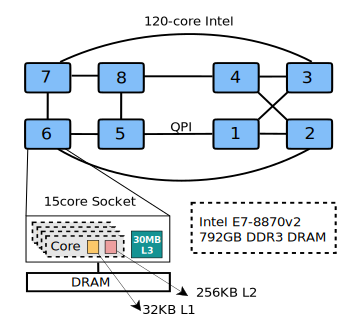
\includegraphics[width=0.4\textwidth]{fig/xeon}
  \end{center}
  \caption{Test-bed Intel xeon archtecture.}
  \label{fig:basic}
\end{figure}
Hyper-Threading is disabled, and Linux kernel 4.5-rc6.
\else

\fi

%$$$$$$$$$$$$$$$$$$$$$$$$$$$$$$$$$$$$$$$$$$$$$$$$$$$$$$$$$$$$$$$$$$$$$$$$$$$$$$$$
%$$$$$$$$$$$$$$$$$$$$$$$$$$$$$$$$$$$$$$$$$$$$$$$$$$$$$$$$$$$$$$$$$$$$$$$$$$$$$$$$
%Benchamrk에 대한 설명
%$$$$$$$$$$$$$$$$$$$$$$$$$$$$$$$$$$$$$$$$$$$$$$$$$$$$$$$$$$$$$$$$$$$$$$$$$$$$$$$$
\ifkor
\noindent
\textbf{Benchmark.} 벤치마크와 워크로드에 대한 BigData Benchmark를 사용하였다.
\begin{itemize}
\item \textbf{Word Count. }We have developed a novel lightweight log-based
structures with efficient log management implementation.
\item \textbf{Grep. }
We applied the in Linux kernel to two reverse mapping(anonymous, file) on
Our design improved throughput and execution time from 1.5x through 2.7x on 120 core.
\item \textbf{Naive Basian. }
We applied the in Linux kernel to two reverse mapping(anonymous, file) on
Our design improved throughput and execution time from 1.5x through 2.7x on 120 core.
\item \textbf{K-means. }
We applied the in Linux kernel to two reverse mapping(anonymous, file) on
Our design improved throughput and execution time from 1.5x through 2.7x on 120 core.
\item \textbf{pagerank. }
We applied the in Linux kernel to two reverse mapping(anonymous, file) on
Our design improved throughput and execution time from 1.5x through 2.7x on 120 core.
\end{itemize}


\else

\fi

\subsection{Spark Scalability Problem}


%$$$$$$$$$$$$$$$$$$$$$$$$$$$$$$$$$$$$$$$$$$$$$$$$$$$$$$$$$$$$$$$$$$$$$$$$$$$$$$$$
%$$$$$$$$$$$$$$$$$$$$$$$$$$$$$$$$$$$$$$$$$$$$$$$$$$$$$$$$$$$$$$$$$$$$$$$$$$$$$$$$
%Scalability 결과에 대한 대략 적인 설명
%$$$$$$$$$$$$$$$$$$$$$$$$$$$$$$$$$$$$$$$$$$$$$$$$$$$$$$$$$$$$$$$$$$$$$$$$$$$$$$$$
\ifkor
Figure 1 shows the spark scalability of five workload.
벤치마크와 워크로드에 대한 BigData Benchmark를 사용하였다.
\else

\fi


%$$$$$$$$$$$$$$$$$$$$$$$$$$$$$$$$$$$$$$$$$$$$$$$$$$$$$$$$$$$$$$$$$$$$$$$$$$$$$$$$
%$$$$$$$$$$$$$$$$$$$$$$$$$$$$$$$$$$$$$$$$$$$$$$$$$$$$$$$$$$$$$$$$$$$$$$$$$$$$$$$$
%CPU utilization에 대한 설명
%$$$$$$$$$$$$$$$$$$$$$$$$$$$$$$$$$$$$$$$$$$$$$$$$$$$$$$$$$$$$$$$$$$$$$$$$$$$$$$$$

\ifkor
벤치마크와 워크로드에 대한 BigData Benchmark를 사용하였다.
\else

\fi


\ifkor
파티션닝 방법이 필요한 이유는 spark library와 runtime엔진이 single node에 동작하는 
시스템의 scalability 특성을 고려하지 않았기 때문이다. 
scale-up server를 위한 spark scalability의 근본적인 해결 방법은 spark library와 
runtime엔진을 scale-up서버를 위해 scalable하게 만드는 것이다.
하지만 scale-out 시스템의 scalability를 위해 작성된 spark의 library와 runtime 엔진을 
수정하는것은 쉽지않다.
이러한 single node로 구성된 manycore scale-up 서버에 대한 scalability
문제는 도커를 활용한 파티셔닝 기법을 사용하여 해결할 수 있다.
이번 장에서는 우리가 수행한 파티션닝 방법이 필요한 이유와 우리가 수행한 방법에 대해서 설명한다.
\else

\fi

%$$$$$$$$$$$$$$$$$$$$$$$$$$$$$$$$$$$$$$$$$$$$$$$$$$$$$$$$$$$$$$$$$$$$$$$$$$$$$$$$
%$$$$$$$$$$$$$$$$$$$$$$$$$$$$$$$$$$$$$$$$$$$$$$$$$$$$$$$$$$$$$$$$$$$$$$$$$$$$$$$$
% NUMA 영향에 대한 설명
%$$$$$$$$$$$$$$$$$$$$$$$$$$$$$$$$$$$$$$$$$$$$$$$$$$$$$$$$$$$$$$$$$$$$$$$$$$$$$$$$
\ifkor
파티션닝 방법이 필요한 가장 큰 이유는 DRAM access latency 때문이다. 
만약 scale-up server가 NUMA 아키텍쳐를 가진 경우일 경우, 
리눅스는 이러한 문제를 해결하기 위해 커널 내부에 automatic NUMA balancing이라는 기능이 있으나, 
아직 파티션되어 수행하는 방법보다는 성능이 떨어진다[]. 그림 xx-xx는 NUMA balancing을 
사용한 방법과 파티션기법을 사용한 방법의 성능 측정한 결과를 보여준다. 
\else

\fi

%$$$$$$$$$$$$$$$$$$$$$$$$$$$$$$$$$$$$$$$$$$$$$$$$$$$$$$$$$$$$$$$$$$$$$$$$$$$$$$$$
%$$$$$$$$$$$$$$$$$$$$$$$$$$$$$$$$$$$$$$$$$$$$$$$$$$$$$$$$$$$$$$$$$$$$$$$$$$$$$$$$
% Linux kernel scalability (lock, cache cohearnci, scheduler)등등 OS 노이즈에 대한 설명
%$$$$$$$$$$$$$$$$$$$$$$$$$$$$$$$$$$$$$$$$$$$$$$$$$$$$$$$$$$$$$$$$$$$$$$$$$$$$$$$$
\ifkor
NUMA의 영향 뿐만 아니라, operating system의 scalability 저해 요소 때문에 파티션닝 방법은 필요하다.
Shared memory 시스템의 공유데이터 때문에 발생하는 scalability 저해 요소 때문에 필요하다.
첫째로 공유 데이터를 lock이 있다. 표 xxx 앞에서 실험한 spark의 wordcount에 대해서 .
JVM 위에서 동작하는 thread간의 공유하는 single address space때문에 발생하는 공유 문제이다.
다음으로 scheduler가 아직 
마지막으로 cache cohearci traffic이 있다. 

\else

\fi


%$$$$$$$$$$$$$$$$$$$$$$$$$$$$$$$$$$$$$$$$$$$$$$$$$$$$$$$$$$$$$$$$$$$$$$$$$$$$$$$$
%$$$$$$$$$$$$$$$$$$$$$$$$$$$$$$$$$$$$$$$$$$$$$$$$$$$$$$$$$$$$$$$$$$$$$$$$$$$$$$$$
% Linux kernel scalability (lock, cache cohearnci, scheduler)등등 OS 노이즈에 대한 설명
%$$$$$$$$$$$$$$$$$$$$$$$$$$$$$$$$$$$$$$$$$$$$$$$$$$$$$$$$$$$$$$$$$$$$$$$$$$$$$$$$
\ifkor
NUMA의 영향 뿐만 아니라, operating system의 scalability 저해 요소 때문에 파티션닝 방법은 필요하다.
Shared memory 시스템의 공유데이터 때문에 발생하는 scalability 저해 요소 때문에 필요하다.
첫째로 공유 데이터를 lock이 있다. 표 xxx 앞에서 실험한 spark의 wordcount에 대해서 .
JVM 위에서 동작하는 thread간의 공유하는 single address space때문에 발생하는 공유 문제이다.
다음으로 scheduler가 아직 
마지막으로 cache cohearci traffic이 있다. 

\else

\fi
